\documentclass[11pt,a4paper,landscape]{article}

\usepackage[margin=0.55in]{geometry}
\usepackage[T1]{fontenc}
\usepackage{lmodern}
\usepackage{tikz}
\usepackage{xcolor}
\usetikzlibrary{arrows.meta,positioning,fit,calc,backgrounds}

\definecolor{ink}{HTML}{102033}
\definecolor{muted}{HTML}{475569}
\definecolor{line}{HTML}{CBD5E1}
\definecolor{panel}{HTML}{F8FAFC}
\definecolor{client}{HTML}{E0F2FE}
\definecolor{clientBorder}{HTML}{0284C7}
\definecolor{server}{HTML}{DCFCE7}
\definecolor{serverBorder}{HTML}{16A34A}
\definecolor{data}{HTML}{FEF3C7}
\definecolor{dataBorder}{HTML}{D97706}
\definecolor{external}{HTML}{F3E8FF}
\definecolor{externalBorder}{HTML}{9333EA}
\definecolor{realtime}{HTML}{FFE4E6}
\definecolor{realtimeBorder}{HTML}{E11D48}

\pagestyle{empty}
\setlength{\parindent}{0pt}

\tikzset{
  font=\sffamily,
  group/.style={
    rounded corners=8pt,
    draw=#1,
    fill=#1!7,
    very thick,
    inner sep=10pt
  },
  box/.style={
    rounded corners=5pt,
    draw=#1,
    fill=white,
    thick,
    align=center,
    minimum width=3.1cm,
    minimum height=1.05cm,
    text=ink
  },
  smallbox/.style={
    rounded corners=5pt,
    draw=#1,
    fill=white,
    thick,
    align=center,
    minimum width=2.75cm,
    minimum height=0.85cm,
    text=ink,
    font=\sffamily\footnotesize
  },
  flow/.style={-{Latex[length=3mm]}, thick, draw=ink},
  dataflow/.style={-{Latex[length=3mm]}, thick, draw=dataBorder},
  realtimeflow/.style={-{Latex[length=3mm]}, thick, draw=realtimeBorder},
  extflow/.style={-{Latex[length=3mm]}, thick, draw=externalBorder},
  note/.style={align=left, text=muted, font=\sffamily\footnotesize}
}

\begin{document}

\begin{center}
  {\LARGE\bfseries IntellMeet System Architecture}\\[2pt]
  {\small React/Vite client, Express API, Socket.IO realtime layer, MongoDB persistence, recordings, transcripts, and AI summaries}
\end{center}

\vspace{0.15cm}

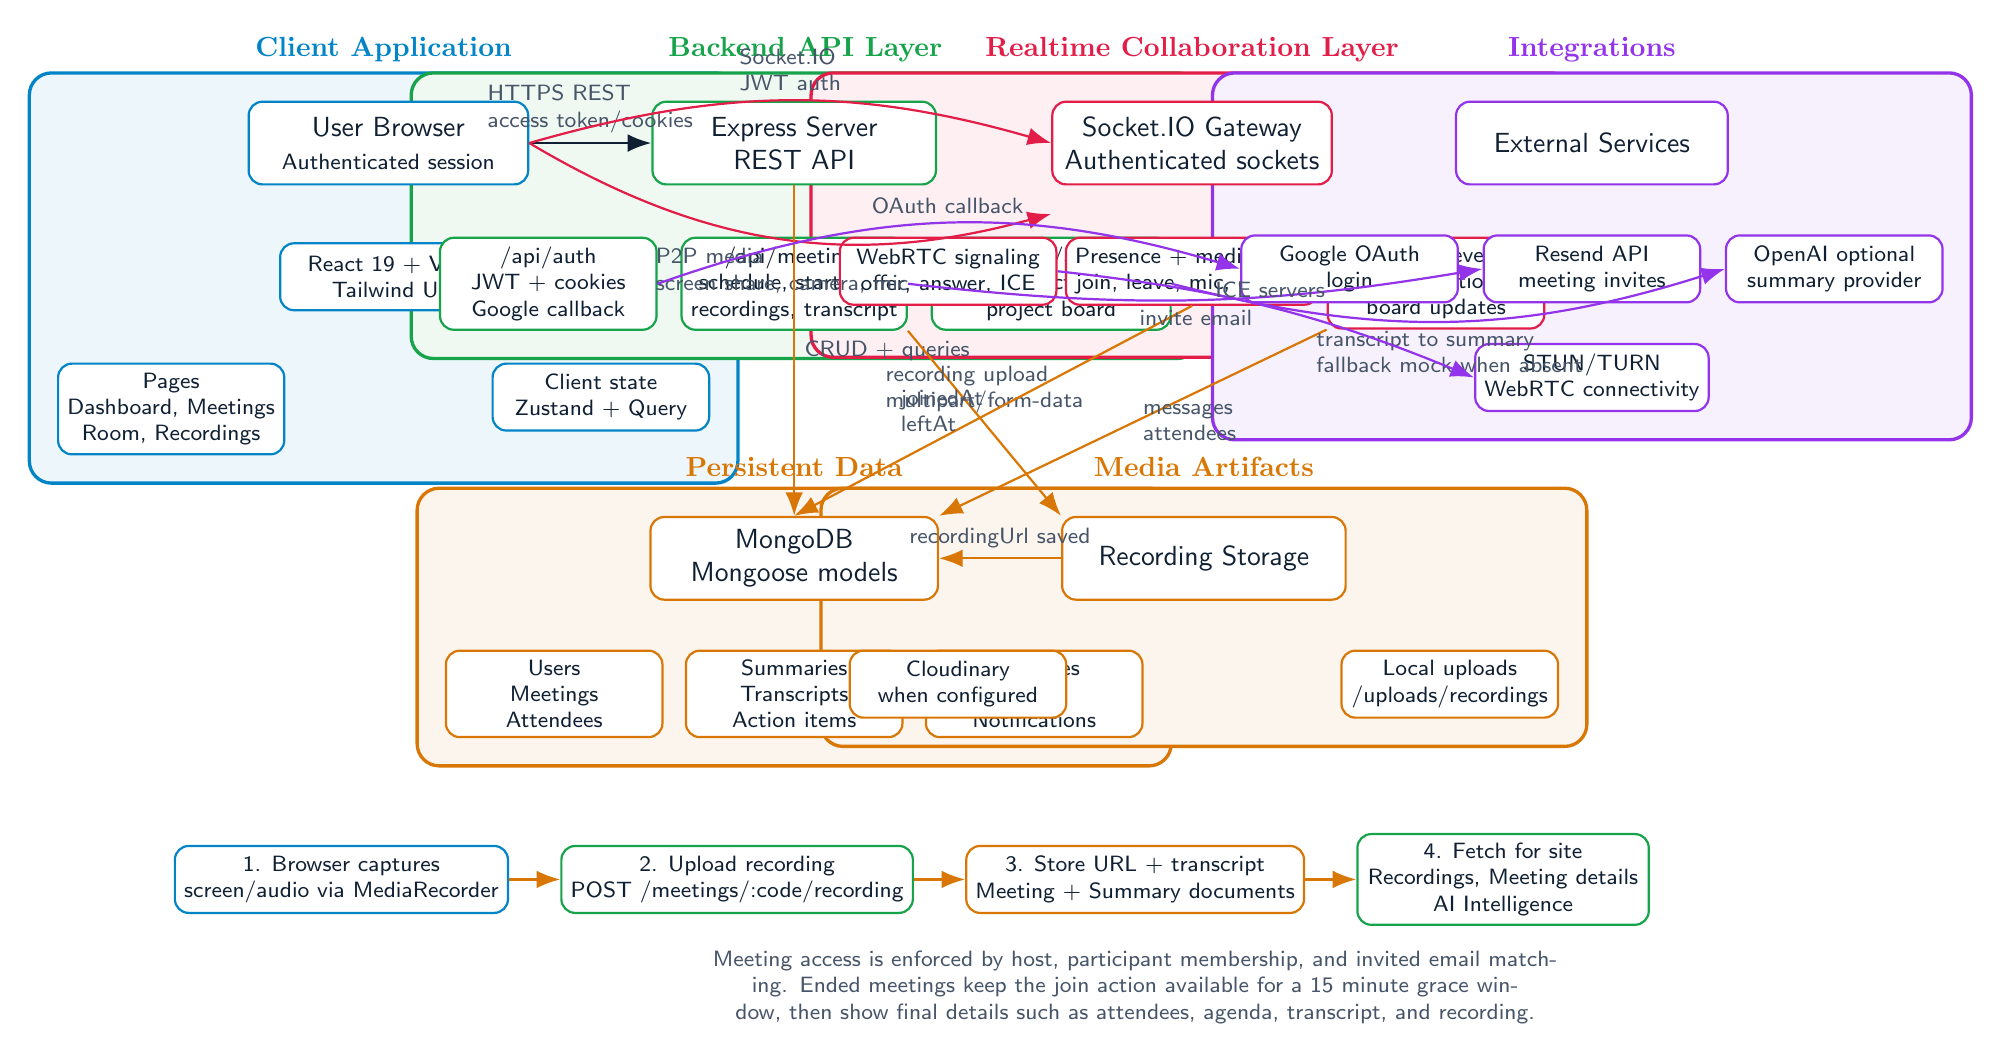
\begin{tikzpicture}[node distance=0.72cm and 1.15cm]

% Client layer
\node[box=clientBorder, minimum width=3.55cm] (browser) {User Browser\\{\footnotesize Authenticated session}};
\node[smallbox=clientBorder, below=of browser] (react) {React 19 + Vite\\Tailwind UI};
\node[smallbox=clientBorder, below left=0.65cm and -0.08cm of react] (pages) {Pages\\Dashboard, Meetings\\Room, Recordings};
\node[smallbox=clientBorder, below right=0.65cm and -0.08cm of react] (clientState) {Client state\\Zustand + Query};

% Backend API
\node[box=serverBorder, right=1.55cm of browser, minimum width=3.6cm] (api) {Express Server\\REST API};
\node[smallbox=serverBorder, below left=0.65cm and -0.08cm of api] (auth) {/api/auth\\JWT + cookies\\Google callback};
\node[smallbox=serverBorder, below=0.65cm of api] (meetingApi) {/api/meetings\\schedule, start, end\\recordings, transcript};
\node[smallbox=serverBorder, below right=0.65cm and -0.08cm of api] (aiApi) {/api/ai + /api/tasks\\summary, action items\\project board};

% Realtime layer
\node[box=realtimeBorder, right=1.45cm of api, minimum width=3.55cm] (socket) {Socket.IO Gateway\\Authenticated sockets};
\node[smallbox=realtimeBorder, below left=0.65cm and -0.08cm of socket] (signal) {WebRTC signaling\\offer, answer, ICE};
\node[smallbox=realtimeBorder, below=0.65cm of socket] (presence) {Presence + media state\\join, leave, mic, camera};
\node[smallbox=realtimeBorder, below right=0.65cm and -0.08cm of socket] (chat) {Realtime events\\chat, captions\\board updates};

% Persistence and storage
\node[box=dataBorder, below=2.35cm of meetingApi, minimum width=3.65cm] (mongo) {MongoDB\\Mongoose models};
\node[smallbox=dataBorder, below left=0.62cm and -0.18cm of mongo] (modelsA) {Users\\Meetings\\Attendees};
\node[smallbox=dataBorder, below=0.62cm of mongo] (modelsB) {Summaries\\Transcripts\\Action items};
\node[smallbox=dataBorder, below right=0.62cm and -0.18cm of mongo] (modelsC) {Messages\\Tasks\\Notifications};

\node[box=dataBorder, right=1.55cm of mongo, minimum width=3.6cm] (storage) {Recording Storage};
\node[smallbox=dataBorder, below left=0.62cm and -0.08cm of storage] (cloudinary) {Cloudinary\\when configured};
\node[smallbox=dataBorder, below right=0.62cm and -0.08cm of storage] (uploads) {Local uploads\\/uploads/recordings};

% External services
\node[box=externalBorder, right=1.55cm of socket, minimum width=3.45cm] (providers) {External Services};
\node[smallbox=externalBorder, below left=0.62cm and -0.05cm of providers] (google) {Google OAuth\\login};
\node[smallbox=externalBorder, below=0.62cm of providers] (resend) {Resend API\\meeting invites};
\node[smallbox=externalBorder, below right=0.62cm and -0.05cm of providers] (openai) {OpenAI optional\\summary provider};
\node[smallbox=externalBorder, below=2.0cm of providers] (stun) {STUN/TURN\\WebRTC connectivity};

\begin{scope}[on background layer]
  \node[group=clientBorder, fit=(browser)(react)(pages)(clientState), label={[font=\bfseries, text=clientBorder]above:Client Application}] {};
  \node[group=serverBorder, fit=(api)(auth)(meetingApi)(aiApi), label={[font=\bfseries, text=serverBorder]above:Backend API Layer}] {};
  \node[group=realtimeBorder, fit=(socket)(signal)(presence)(chat), label={[font=\bfseries, text=realtimeBorder]above:Realtime Collaboration Layer}] {};
  \node[group=dataBorder, fit=(mongo)(modelsA)(modelsB)(modelsC), label={[font=\bfseries, text=dataBorder]above:Persistent Data}] {};
  \node[group=dataBorder, fit=(storage)(cloudinary)(uploads), label={[font=\bfseries, text=dataBorder]above:Media Artifacts}] {};
  \node[group=externalBorder, fit=(providers)(google)(resend)(openai)(stun), label={[font=\bfseries, text=externalBorder]above:Integrations}] {};
\end{scope}

% Main flows
\draw[flow] (browser.east) -- node[above, note] {HTTPS REST\\access token/cookies} (api.west);
\draw[realtimeflow] (browser.east) to[bend left=16] node[above, note] {Socket.IO\\JWT auth} (socket.west);
\draw[realtimeflow] (browser.east) to[bend right=23] node[below, note] {P2P media\\screen share, camera, mic} ($(socket.west)+(0,-0.9)$);

\draw[dataflow] (api.south) -- node[right, note] {CRUD + queries} (mongo.north);
\draw[dataflow] (meetingApi.south east) -- node[above, note] {recording upload\\multipart/form-data} (storage.north west);
\draw[dataflow] (storage.west) -- node[above, note] {recordingUrl saved} (mongo.east);
\draw[dataflow] (chat.south west) -- node[right, note] {messages\\attendees} (mongo.north east);
\draw[dataflow] (presence.south) -- node[left, note] {joinedAt\\leftAt} (mongo.north);

\draw[extflow] (auth.east) to[bend left=18] node[above, note] {OAuth callback} (google.west);
\draw[extflow] (meetingApi.east) to[bend right=8] node[below, note] {invite email} (resend.west);
\draw[extflow] (aiApi.east) to[bend right=16] node[below, note] {transcript to summary\\fallback mock when absent} (openai.west);
\draw[extflow] (signal.east) to[bend left=8] node[above, note] {ICE servers} (stun.west);

% Recording/transcript sequence strip
\node[smallbox=clientBorder, minimum width=3.7cm, below=3.1cm of mongo, xshift=-5.75cm] (capture) {1. Browser captures\\screen/audio via MediaRecorder};
\node[smallbox=serverBorder, minimum width=3.7cm, right=0.65cm of capture] (upload) {2. Upload recording\\POST /meetings/:code/recording};
\node[smallbox=dataBorder, minimum width=3.7cm, right=0.65cm of upload] (persist) {3. Store URL + transcript\\Meeting + Summary documents};
\node[smallbox=serverBorder, minimum width=3.7cm, right=0.65cm of persist] (fetch) {4. Fetch for site\\Recordings, Meeting details\\AI Intelligence};

\draw[dataflow] (capture) -- (upload);
\draw[dataflow] (upload) -- (persist);
\draw[dataflow] (persist) -- (fetch);

\node[note, below=0.35cm of persist, text width=12.2cm, align=center] {
Meeting access is enforced by host, participant membership, and invited email matching. Ended meetings keep the join action available for a 15 minute grace window, then show final details such as attendees, agenda, transcript, and recording.
};

\end{tikzpicture}

\vfill
\begin{center}
  {\footnotesize Overleaf usage: create a new project, paste this file as \texttt{architecture-diagram.tex}, then compile with pdfLaTeX.}
\end{center}

\end{document}
